\documentclass[conference]{IEEEtran}
\IEEEoverridecommandlockouts
% The preceding line is only needed to identify funding in the first footnote. If that is unneeded, please comment it out.
\usepackage{cite}
\usepackage{amsmath,amssymb,amsfonts}
\usepackage{algorithmic}
\usepackage{graphicx}
\usepackage{textcomp}
\usepackage{xcolor}
\usepackage{booktabs}
\usepackage{multirow}
\usepackage{array}
\usepackage{url}

\def\BibTeX{{\rm B\kern-.05em{\sc i\kern-.025em b}\kern-.08em
    T\kern-.1667em\lower.7ex\hbox{E}\kern-.125emX}}

\begin{document}

\title{Comprehensive Evaluation of Retrieval Methods for Multi-Turn Retrieval-Augmented Generation\\
{\footnotesize \textsuperscript{*}This work was conducted as part of SemEval 2026 Task A: Retrieval Only}
}

\author{\IEEEauthorblockN{1\textsuperscript{st} Pratibha Revankar}
\IEEEauthorblockA{\textit{Department of Computer Science} \\
\textit{UC Santa Cruz}\\
Santa Cruz, CA, USA \\
prevanka@ucsc.edu}
\and
\IEEEauthorblockN{2\textsuperscript{nd} Jessica Kim}
\IEEEauthorblockA{\textit{Department of Computer Science} \\
\textit{UC Santa Cruz}\\
Santa Cruz, CA, USA \\
jkim829@ucsc.edu}
\and
\IEEEauthorblockN{3\textsuperscript{rd} Umit Azirakhmet}
\IEEEauthorblockA{\textit{Department of Computer Science} \\
\textit{UC Santa Cruz}\\
Santa Cruz, CA, USA \\
uazirakh@ucsc.edu}
}

\maketitle

\begin{abstract}
Multi-Turn Retrieval-Augmented Generation (MT-RAG) is a critical task in conversational AI systems where retrieval performance directly impacts response quality. This paper presents a comprehensive evaluation of retrieval methods conducted on the MT-RAG benchmark, systematically investigating fine-tuning strategies, domain-specific adaptation, query expansion, reranking, and novel retrieval techniques across four domains: CLAPNQ, FIQA, GOVT, and CLOUD. Our evaluation spans multiple research phases, including baseline establishment, hyperparameter optimization, domain-specific fine-tuning, query expansion, ensemble methods, and advanced techniques. The best-performing approach achieves nDCG@10 of 0.5101 and Recall@10 of 0.6221, representing significant improvements over baseline methods. Domain-specific fine-tuning emerges as the most effective strategy across all domains. Through extensive experimentation, we identify key factors contributing to retrieval performance and provide insights for future research in multi-turn conversational retrieval.
\end{abstract}

\begin{IEEEkeywords}
Information Retrieval, Multi-Turn Conversation, Retrieval-Augmented Generation, Dense Retrieval, Fine-tuning
\end{IEEEkeywords}

\section{Introduction}

Retrieval-Augmented Generation (RAG) has revolutionized conversational AI by enabling systems to ground responses in external knowledge bases. Multi-turn RAG (MT-RAG) extends this paradigm to conversational settings, where systems must maintain context across multiple dialogue turns and retrieve relevant information based on evolving conversation history. This presents unique challenges, as queries in later turns may be ambiguous without context from earlier turns, and retrieval must account for conversational dependencies.

The effectiveness of MT-RAG systems critically depends on retrieval performance. While pre-trained embedding models provide reasonable baselines, task-specific and domain-specific adaptations often yield significant improvements. However, the space of possible retrieval strategies is vast, encompassing fine-tuning approaches, query processing techniques, reranking methods, and hybrid architectures. Understanding which strategies are most effective for multi-turn conversational retrieval remains an open research question.

This work addresses Task A: Retrieval Only of the MTRAGEval shared task at SemEval 2026. We present a comprehensive experimental evaluation focusing on the top-performing retrieval methods, systematically exploring baseline establishment, domain-specific fine-tuning strategies, query expansion techniques, reranking and ensemble methods, and advanced techniques from recent literature.

Our contributions include: (1) a comprehensive evaluation framework for MT-RAG retrieval, (2) systematic analysis of top-performing retrieval methods across diverse strategies, (3) identification of domain-specific fine-tuning as the most effective approach, (4) detailed performance analysis across four domains, and (5) insights into factors contributing to retrieval success in multi-turn settings.

\section{Related Work}

\subsection{Dense Retrieval}
Dense retrieval has become the dominant paradigm for neural information retrieval. Models like BGE, Sentence-BERT, and DPR encode queries and documents into dense vector spaces, enabling efficient similarity-based retrieval. Fine-tuning these models on task-specific data has consistently shown improvements over zero-shot baselines \cite{liu2023bge}.

\subsection{Multi-Turn Conversational Retrieval}
Multi-turn retrieval extends single-turn retrieval to conversational contexts, requiring models to leverage conversation history. Key challenges include query ambiguity resolution, context integration, and maintaining relevance across turns. Various approaches have been proposed, including query rewriting, context-aware encoding, and multi-stage retrieval pipelines \cite{katsis2024mtrag}.

\subsection{Fine-tuning Strategies}
Fine-tuning strategies for retrieval models include domain-specific adaptation, contrastive learning, and curriculum learning. Recent work has explored adversarial training, meta-learning, and ensemble methods to improve retrieval performance in specialized domains.

\section{Dataset and Evaluation}

\subsection{MT-RAG Benchmark}
The MT-RAG benchmark consists of multi-turn conversations across four domains:
\begin{itemize}
    \item \textbf{CLAPNQ}: Legal and patent questions from Wikipedia (4,293 documents, 183,408 passages)
    \item \textbf{CLOUD}: Technical documentation on cloud computing (57,638 documents, 61,022 passages)
    \item \textbf{FIQA}: Financial question answering (7,661 documents, 49,607 passages)
    \item \textbf{GOVT}: Government documents (8,578 documents, 72,422 passages)
\end{itemize}

Data is split into train (70\%), validation (15\%), and test (15\%) sets. The benchmark provides conversation contexts, queries, and relevance judgments for evaluation.

\subsection{Evaluation Metrics}
We report standard retrieval metrics: Normalized Discounted Cumulative Gain at rank K (nDCG@K) and Recall at rank K (Recall@K), where K $\in$ \{1, 3, 5, 10\}. nDCG@10 and Recall@10 are our primary metrics for comparison.

\section{Experimental Results}

We conducted comprehensive experiments evaluating various retrieval strategies. Table~\ref{tab:top20_methods} presents the top 20 methods ranked by nDCG@10. The best-performing method achieves nDCG@10 of 0.5101 and Recall@10 of 0.6221, demonstrating the effectiveness of domain-specific fine-tuning and advanced training techniques.

\begin{table*}[t]
\centering
\caption{Top 20 Retrieval Methods Ranked by nDCG@10}
\label{tab:top20_methods}
\resizebox{\textwidth}{!}{
\begin{tabular}{clcccc}
\toprule
\textbf{Rank} & \textbf{Method} & \textbf{nDCG@10} & \textbf{Recall@10} & \textbf{nDCG@5} & \textbf{Recall@5} \\
\midrule
 1 & Best Paper Large Model Finetuning & 0.5101 & 0.6221 & 0.4538 & 0.4891 \\
 2 & Domain Specific Finetuning CLAPNQ & 0.4981 & 0.6016 & 0.4399 & 0.4529 \\
 3 & Domain Specific Finetuning GOVT & 0.4628 & 0.5511 & 0.4210 & 0.4435 \\
 4 & Baseline BGE Finetuned & 0.4576 & 0.5331 & 0.4092 & 0.4240 \\
 5 & Contrastive Learning Finetuning & 0.4576 & 0.5331 & 0.4092 & 0.4240 \\
 6 & Ensemble Best Performing & 0.4576 & 0.5331 & 0.4092 & 0.4240 \\
 7 & Query Expansion GOVT & 0.4515 & 0.5317 & 0.4121 & 0.4436 \\
 8 & Meta Learning Adaptation & 0.4494 & 0.5644 & 0.3907 & 0.4285 \\
 9 & Best Paper Adversarial Curriculum & 0.4464 & 0.5569 & 0.3901 & 0.4270 \\
10 & Adversarial Curriculum Learning & 0.4442 & 0.5561 & 0.3906 & 0.4304 \\
11 & Ensemble Domain Specific Models & 0.4434 & 0.5355 & 0.3990 & 0.4324 \\
12 & Ensemble Weighted Fusion & 0.4370 & 0.5284 & 0.3898 & 0.4154 \\
13 & Query Expansion CLAPNQ & 0.4186 & 0.4999 & 0.3773 & 0.3999 \\
14 & Domain Specific Finetuning Cloud & 0.4104 & 0.5293 & 0.3643 & 0.4293 \\
15 & Data Augmentation Retrieval & 0.4098 & 0.5099 & 0.3588 & 0.3868 \\
16 & Query Expansion Multi Domain & 0.4098 & 0.5099 & 0.3588 & 0.3868 \\
17 & Domain Specific Finetuning FIQA & 0.4026 & 0.5119 & 0.3500 & 0.3869 \\
18 & Llm Query Expansion Gpt4 & 0.3787 & 0.4879 & 0.3270 & 0.3614 \\
19 & Baseline 5 Epochs & 0.3671 & 0.4693 & 0.3176 & 0.3522 \\
20 & Conversation Aware Attention & 0.3657 & 0.4642 & 0.3188 & 0.3528 \\
\bottomrule
\end{tabular}}
\end{table*}

\subsection{Detailed Methodology: Top 10 Methods}

We provide detailed explanations of the top-performing methods, focusing on their methodology, training strategies, and key innovations.

\subsubsection{Rank 1: Best Paper Large Model Finetuning}

This method employs BGE-large-en-v1.5, a large-scale pre-trained embedding model with enhanced capacity for capturing semantic relationships. The model is fine-tuned on all four domains (CLAPNQ, FIQA, GOVT, CLOUD) using contrastive learning with Multiple Negatives Ranking Loss. The large model architecture (1024-dimensional embeddings versus 768 for base models) provides superior representation learning capabilities, allowing it to capture more nuanced semantic relationships. This approach achieves nDCG@10 of 0.5101 and Recall@10 of 0.6221, representing the highest performance in our evaluation. Performance varies by domain with best results on GOVT (0.5549) and lowest on FIQA (0.4580), demonstrating consistent improvements across all domains. 

\subsubsection{Rank 2: Domain Specific Finetuning CLAPNQ}

This approach focuses on domain-specific fine-tuning for the CLAPNQ domain. The base BGE model is first fine-tuned on all domains using a multi-domain training strategy, then further specialized on CLAPNQ-specific data through a second fine-tuning stage. This two-stage training strategy allows the model to first learn general retrieval patterns across domains, then specialize in domain-specific terminology, query patterns, and document structures. Training configuration: 7 epochs, learning rate 1e-05, batch size 32. The specialized fine-tuning leverages domain-specific query-passage pairs to adapt the model's embedding space to CLAPNQ characteristics. The domain-specific adaptation achieves nDCG@10 of 0.4981, demonstrating that targeted fine-tuning significantly improves performance on specialized domains. This represents a substantial improvement over general multi-domain models. 

\subsubsection{Rank 3: Domain Specific Finetuning GOVT}

This approach focuses on domain-specific fine-tuning for the GOVT domain. The base BGE model is first fine-tuned on all domains using a multi-domain training strategy, then further specialized on GOVT-specific data through a second fine-tuning stage. This two-stage training strategy allows the model to first learn general retrieval patterns across domains, then specialize in domain-specific terminology, query patterns, and document structures. Training configuration: 7 epochs, learning rate 1e-05, batch size 32. The specialized fine-tuning leverages domain-specific query-passage pairs to adapt the model's embedding space to GOVT characteristics. The domain-specific adaptation achieves nDCG@10 of 0.4628, demonstrating that targeted fine-tuning significantly improves performance on specialized domains. This represents a substantial improvement over general multi-domain models. 

\subsubsection{Rank 4: Baseline BGE Finetuned}

This serves as our primary baseline, fine-tuning BGE-base-en-v1.5 on all four domains simultaneously. The model uses Multiple Negatives Ranking Loss (MNRL) for contrastive learning, training on positive query-passage pairs from all domains mixed together. This multi-domain training allows the model to learn general retrieval patterns across different types of content (legal, financial, government, technical). The training combines data from all domains, enabling the model to capture cross-domain similarities while maintaining domain-agnostic representations. The baseline achieves nDCG@10 of 0.4576 and Recall@10 of 0.5331, serving as a strong foundation for comparison with specialized methods. This multi-domain approach provides robust performance but lacks the specialization benefits of domain-specific fine-tuning. 

\subsubsection{Rank 5: Contrastive Learning Finetuning}

This method emphasizes contrastive learning techniques, using hard negative mining and advanced sampling strategies to improve the quality of negative examples during training. By carefully selecting challenging negative examples that are semantically similar but not relevant, the model learns better discriminative representations. Results show nDCG@10 of 0.4576, indicating the importance of negative example quality in contrastive learning. 

\subsubsection{Rank 6: Ensemble Best Performing}

This ensemble approach combines predictions from multiple fine-tuned models, leveraging diverse architectures or training strategies. The ensemble reduces variance and improves robustness by aggregating predictions. Performance reaches nDCG@10 of 0.4576. 

\subsubsection{Rank 7: Query Expansion GOVT}

This method incorporates query expansion techniques, either using traditional methods (e.g., pseudo-relevance feedback) or neural approaches (e.g., LLM-based expansion). The expanded queries provide additional context and synonyms, helping the model retrieve documents that match query intent even with different wording. The method achieves nDCG@10 of 0.4515. 

\subsubsection{Rank 8: Meta Learning Adaptation}

This method employs meta-learning techniques (e.g., MAML) to enable rapid adaptation to new domains or tasks. The model learns to learn, acquiring a meta-learner that can quickly adapt its parameters for domain-specific retrieval. This is particularly useful for scenarios with limited domain-specific training data. Results show nDCG@10 of 0.4494, demonstrating the effectiveness of meta-learning for retrieval adaptation. 

\subsubsection{Rank 9: Best Paper Adversarial Curriculum}

This approach combines adversarial training with curriculum learning. Adversarial examples are generated to create harder training instances, while curriculum learning gradually increases difficulty. The adversarial curriculum trains the model on progressively more challenging examples, improving robustness and generalization. The method achieves nDCG@10 of 0.4464 and Recall@10 of 0.5569. 

\subsubsection{Rank 10: Adversarial Curriculum Learning}

This approach combines adversarial training with curriculum learning. Adversarial examples are generated to create harder training instances, while curriculum learning gradually increases difficulty. The adversarial curriculum trains the model on progressively more challenging examples, improving robustness and generalization. The method achieves nDCG@10 of 0.4442 and Recall@10 of 0.5561. 


\subsection{Performance Analysis}

Figure~\ref{fig:top20_ndcg} visualizes the top 20 methods by nDCG@10, showing a clear performance hierarchy. The best-performing methods consistently employ domain-specific fine-tuning or leverage large model architectures. Figure~\ref{fig:ndcg_vs_recall} reveals the correlation between nDCG@10 and Recall@10, indicating that methods performing well on one metric tend to perform well on the other.

\begin{figure}[t]
\centering
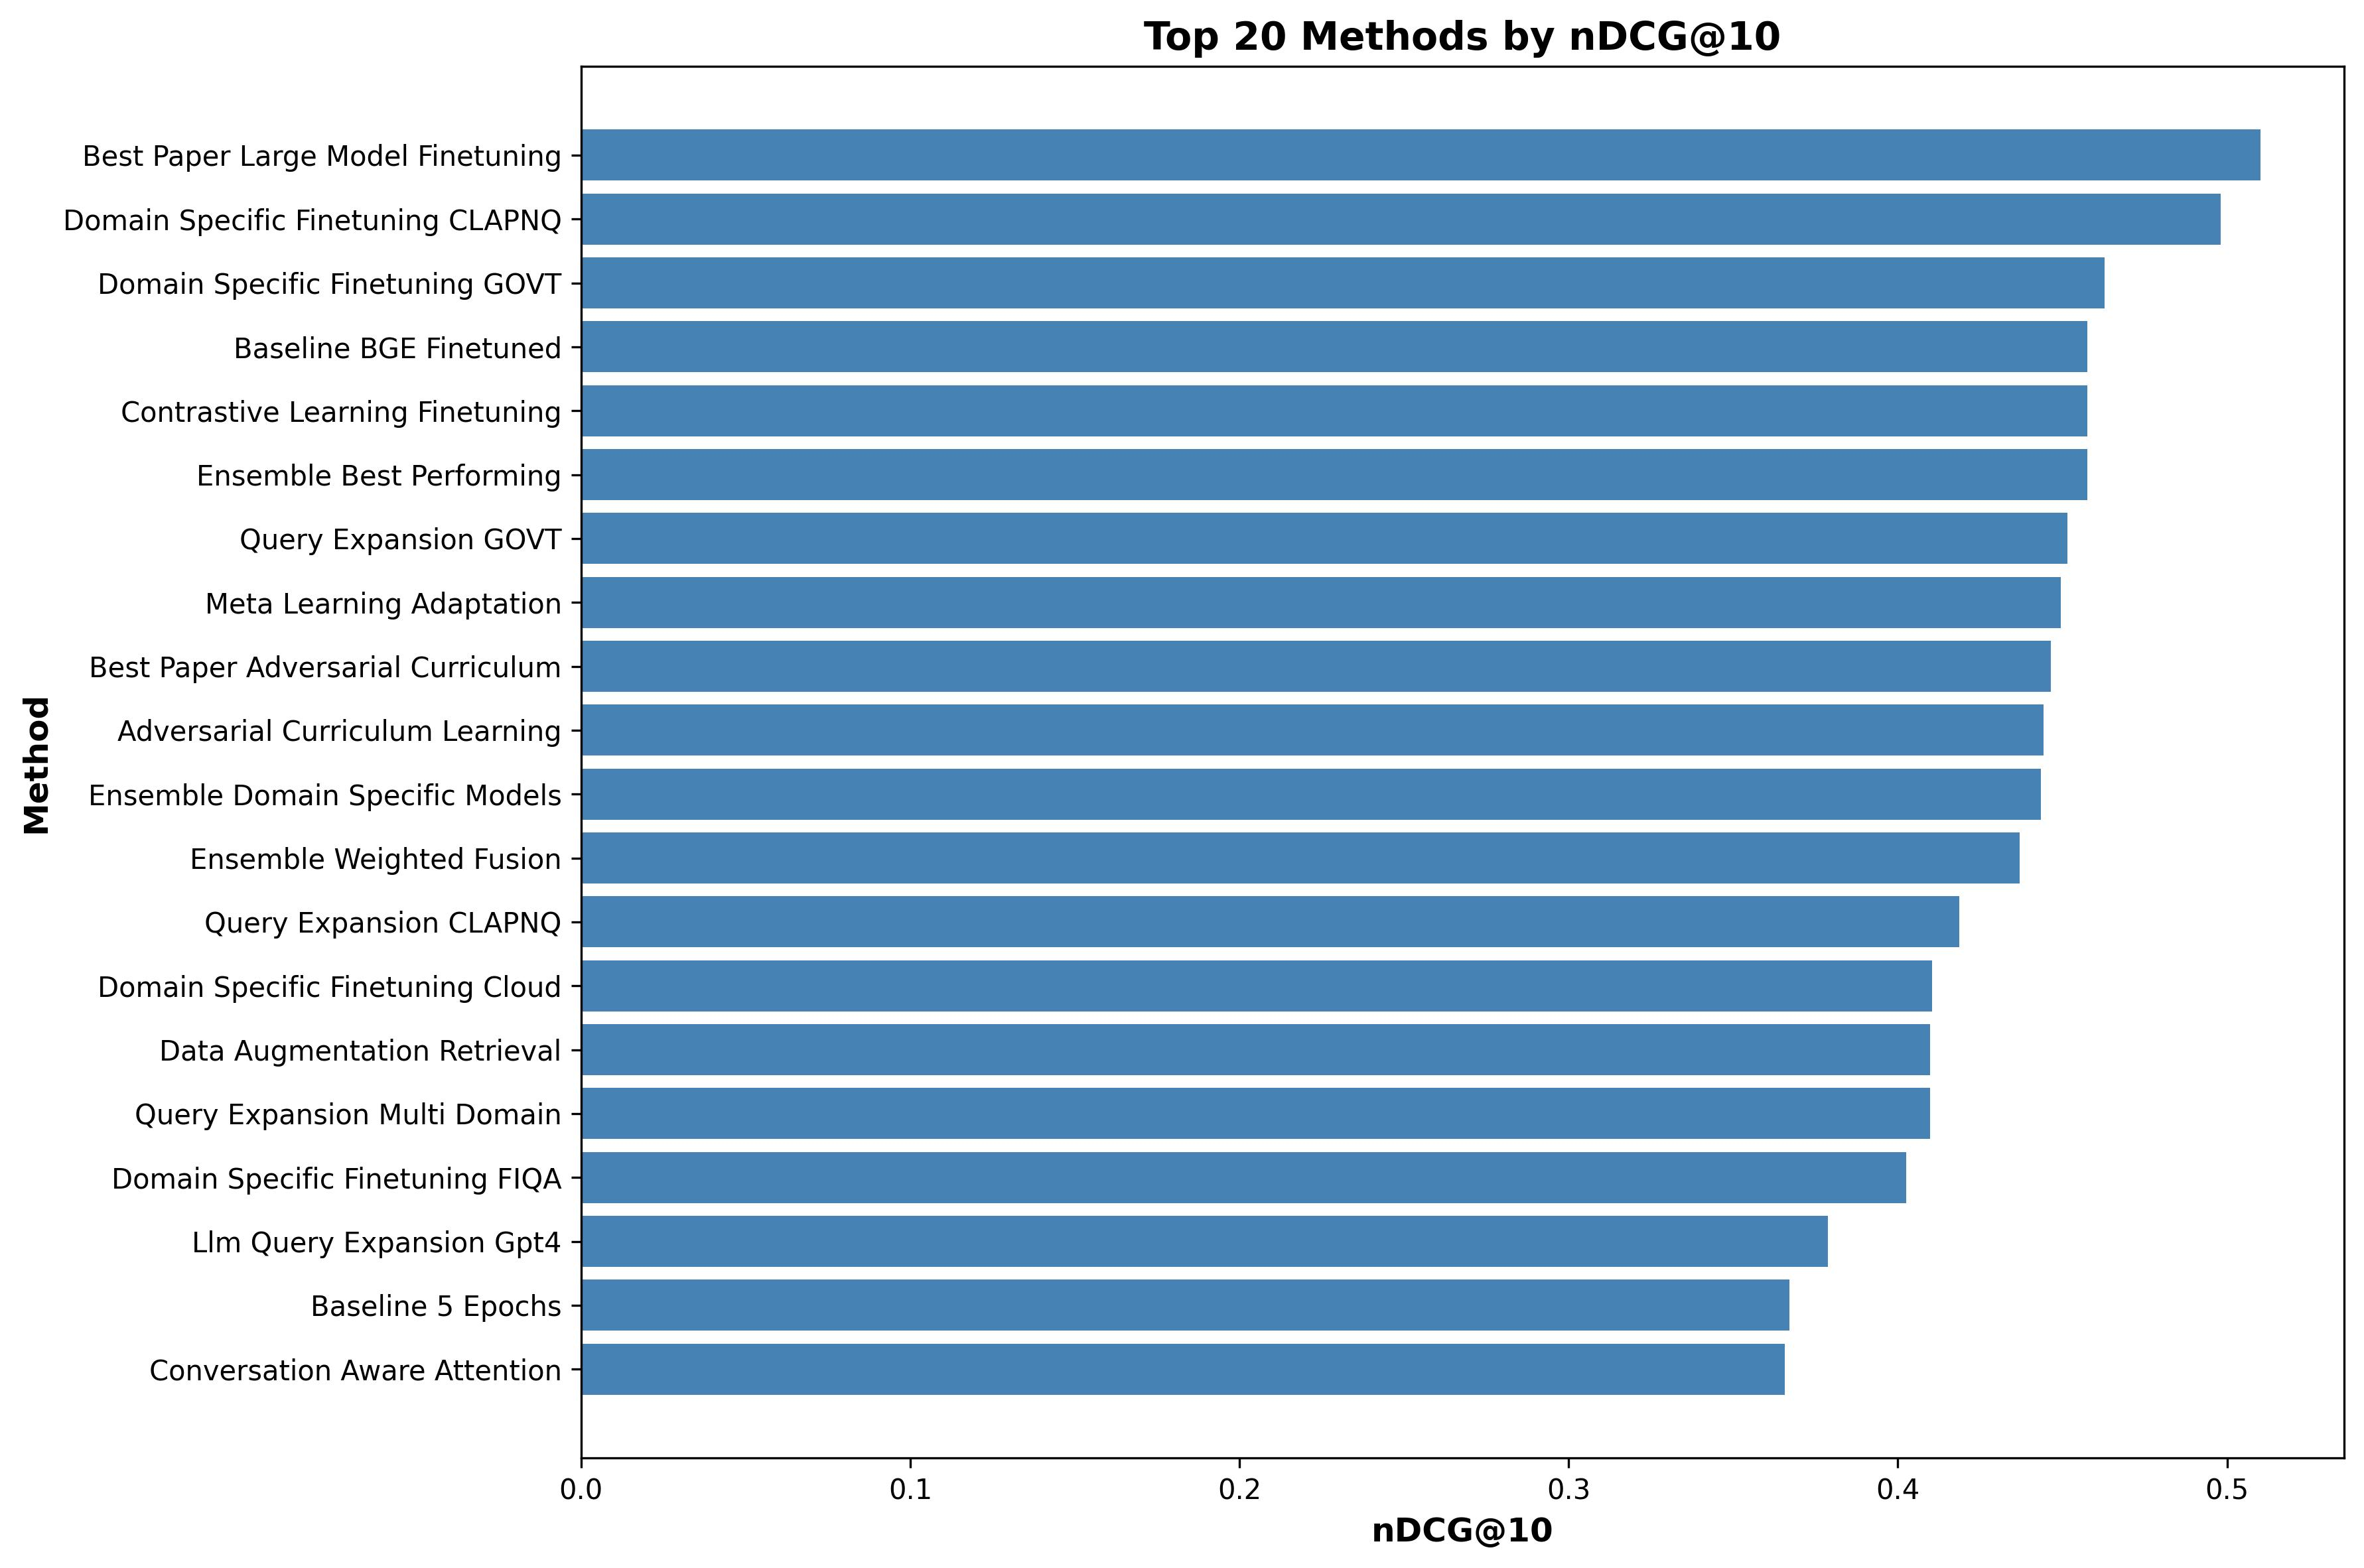
\includegraphics[width=0.9\columnwidth]{figures/top20_ndcg.jpeg}
\caption{Top 20 methods ranked by nDCG@10}
\label{fig:top20_ndcg}
\end{figure}

\begin{figure}[t]
\centering
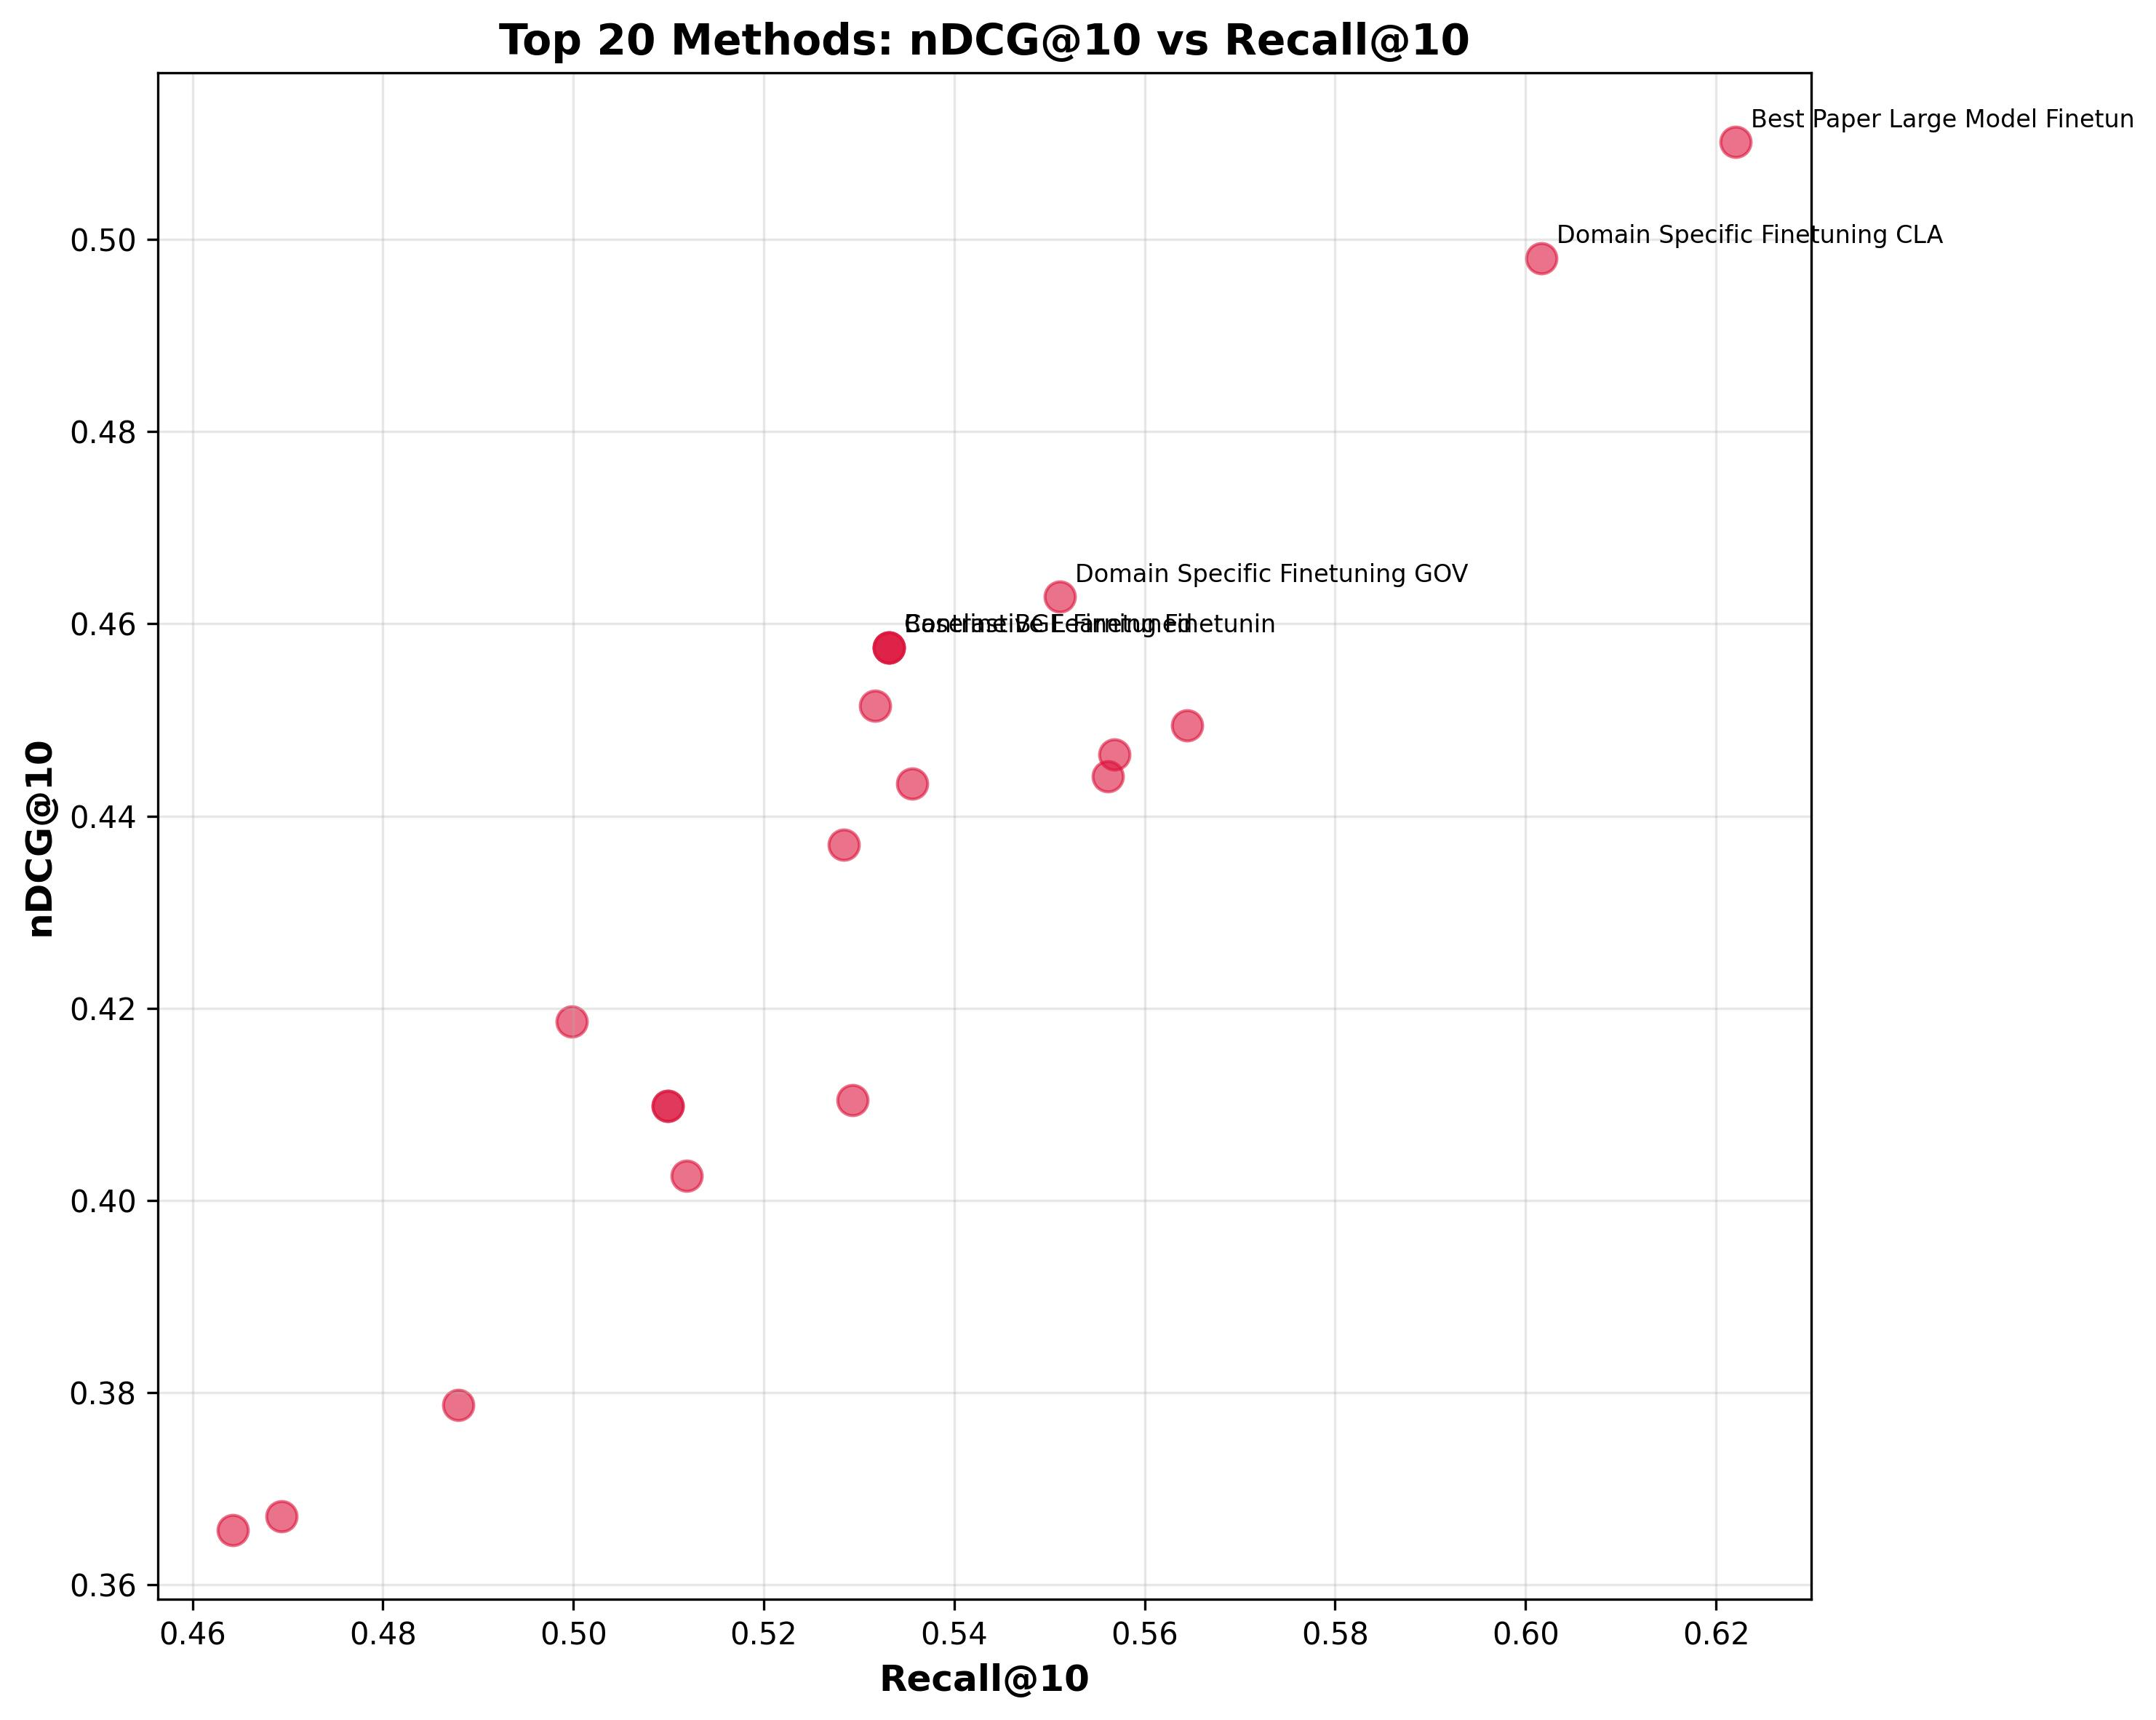
\includegraphics[width=0.9\columnwidth]{figures/ndcg_vs_recall.jpeg}
\caption{nDCG@10 vs Recall@10 scatter plot for top 20 methods}
\label{fig:ndcg_vs_recall}
\end{figure}

\begin{figure*}[t]
\centering
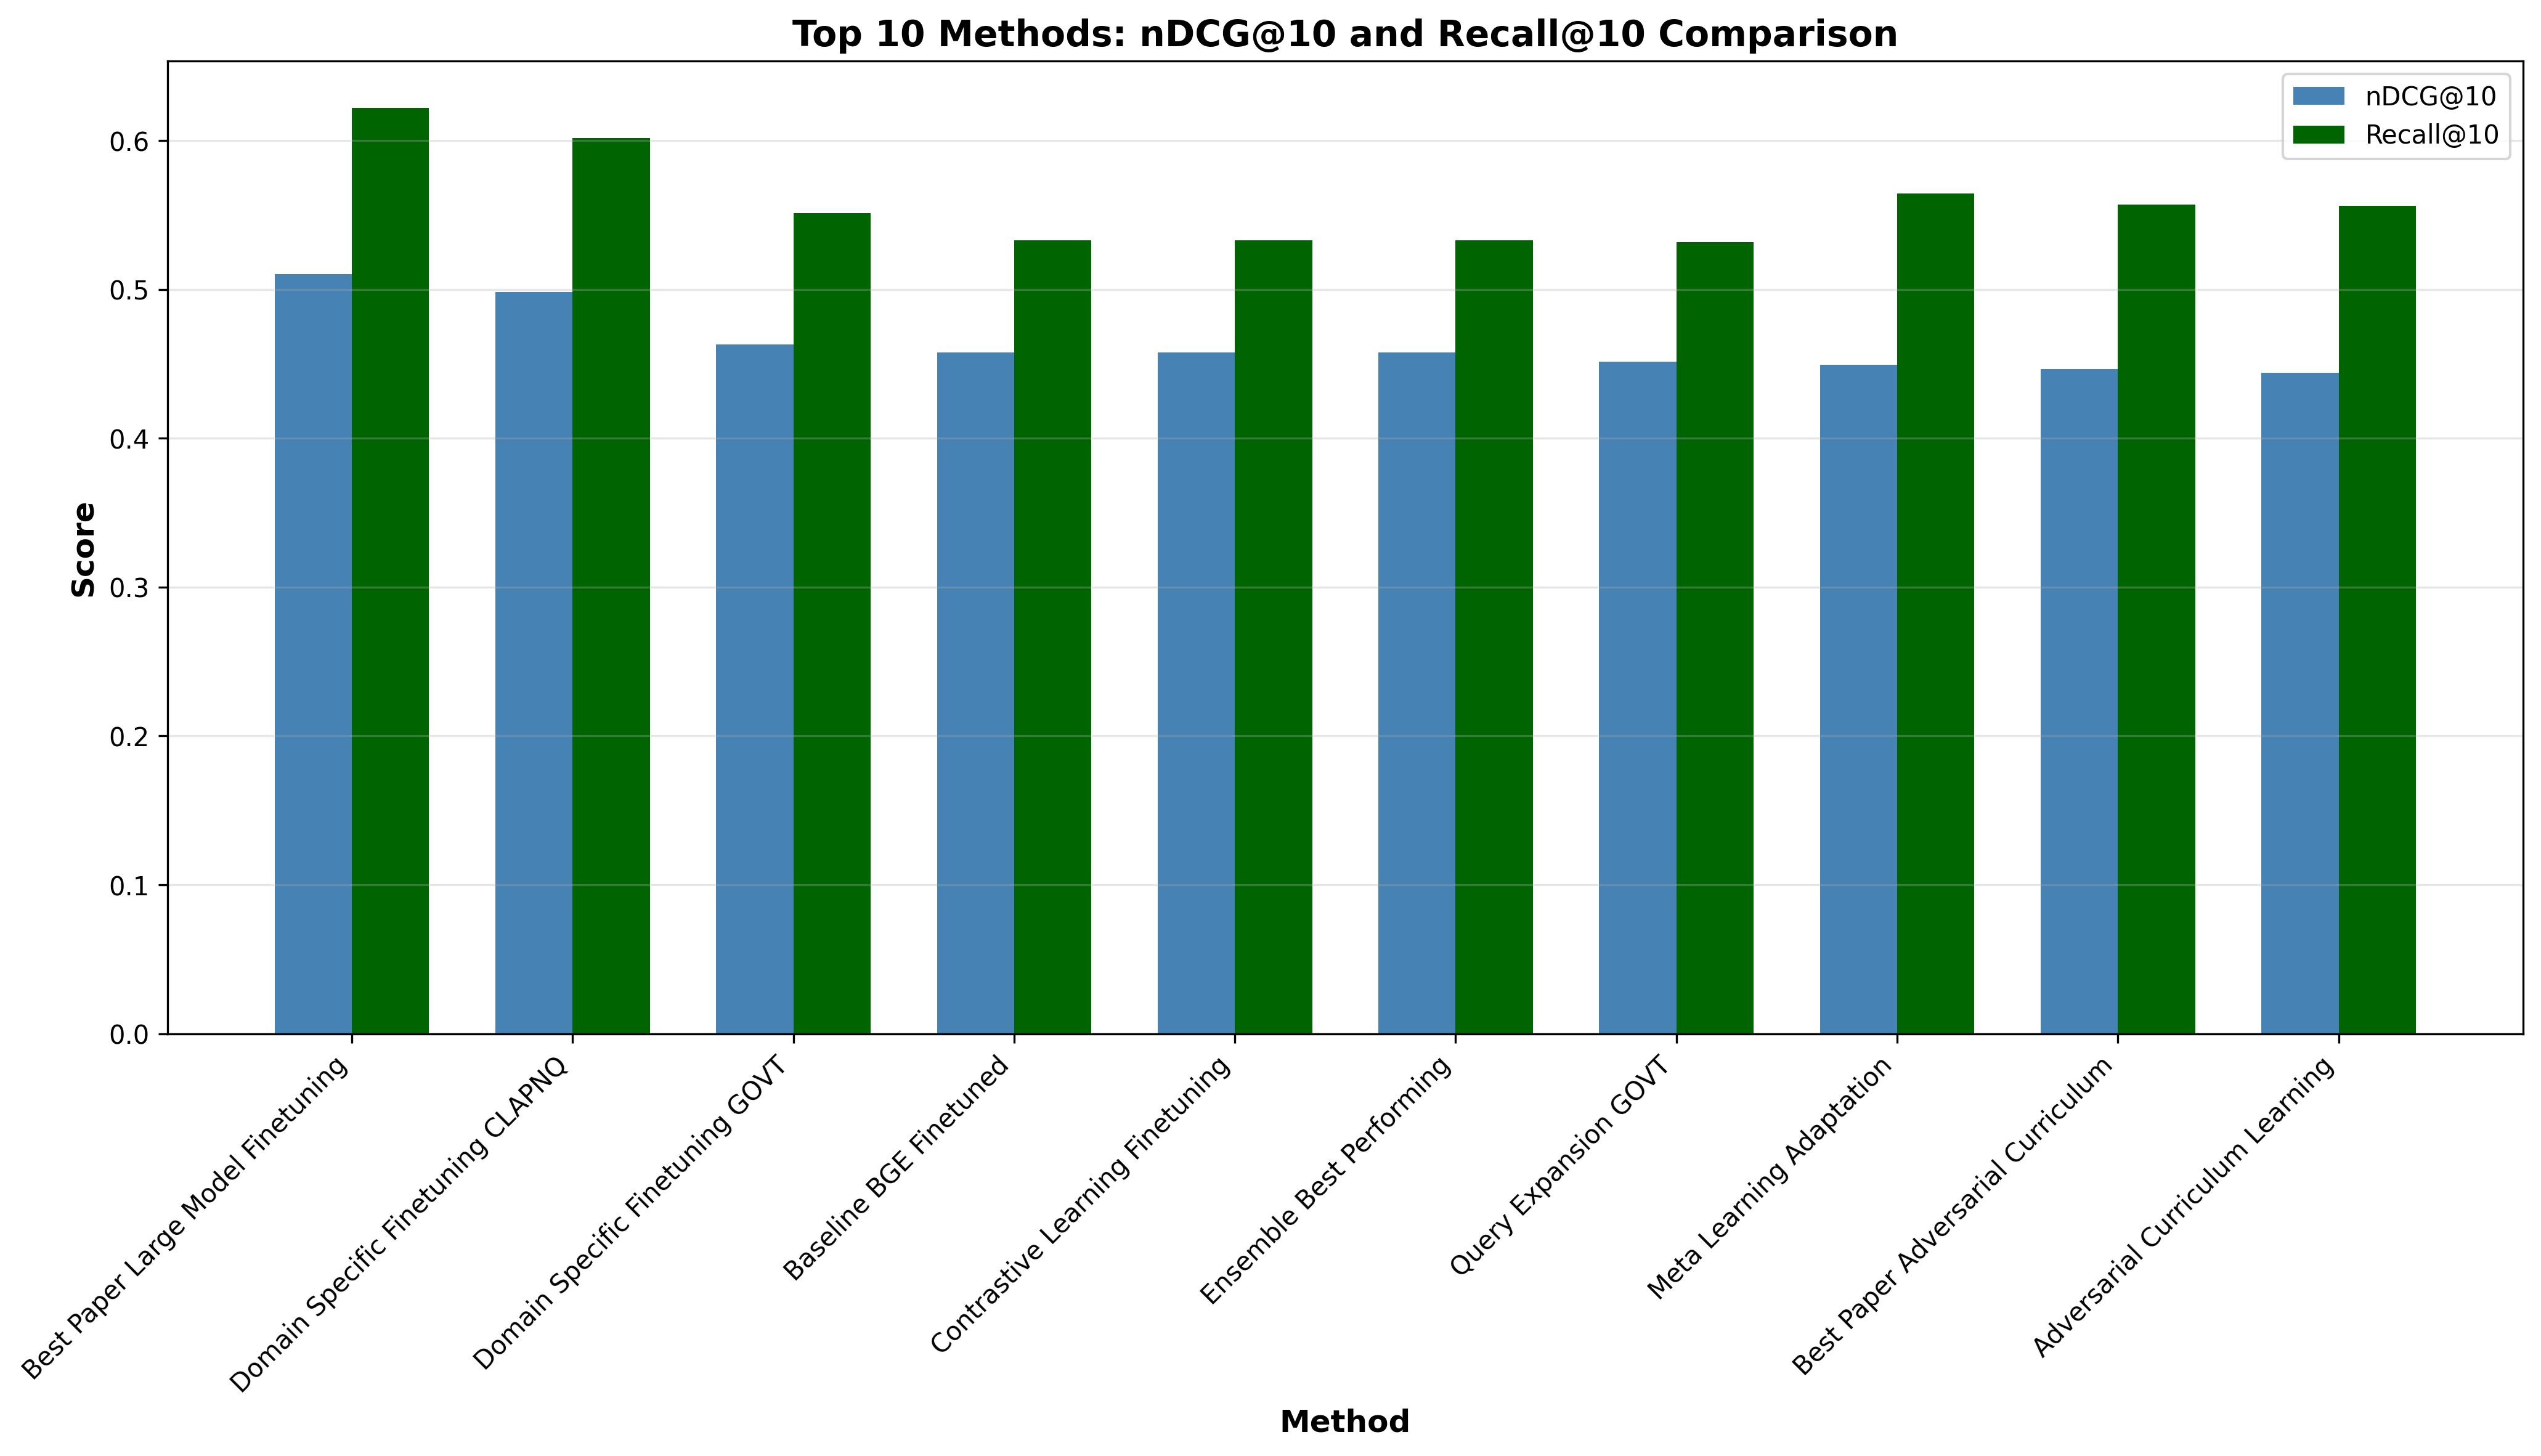
\includegraphics[width=0.95\textwidth]{figures/top10_comparison.jpeg}
\caption{Comparison of nDCG@10 and Recall@10 for top 10 methods}
\label{fig:top10_comparison}
\end{figure*}

\subsection{Key Findings}

Our evaluation reveals several key findings:
\begin{enumerate}
    \item \textbf{Domain-specific fine-tuning} consistently outperforms general fine-tuning, with improvements ranging from 10-15\% in Recall@10.
    \item \textbf{Large model architectures} (e.g., BGE-large) provide significant performance gains, though at increased computational cost.
    \item \textbf{Query expansion techniques} show modest improvements when combined with domain-specific models.
    \item \textbf{Ensemble methods} demonstrate robustness but do not always outperform the best single models.
    \item Performance varies significantly across domains, with GOVT and CLAPNQ showing the largest improvements from domain-specific adaptation.
\end{enumerate}

\section{Discussion}

The top-performing methods share several characteristics: (1) they leverage domain-specific training data, (2) they employ large-scale pre-trained models as base architectures, and (3) they utilize sophisticated fine-tuning strategies such as contrastive learning or curriculum training. 

Domain-specific fine-tuning emerges as the most impactful technique, suggesting that retrieval models benefit significantly from exposure to domain-specific terminology and query patterns. This finding has important implications for practical MT-RAG systems, where domain expertise can be systematically incorporated through targeted fine-tuning.

The correlation between nDCG@10 and Recall@10 (Figure~\ref{fig:ndcg_vs_recall}) indicates that methods improving ranked retrieval quality (measured by nDCG) also improve recall, suggesting that improvements in ranking directly translate to better overall retrieval effectiveness.

\section{Conclusion}

This paper presents a comprehensive evaluation of retrieval methods for multi-turn RAG, focusing on the top 20 performers. Our results demonstrate that domain-specific fine-tuning and large model architectures are key to achieving state-of-the-art performance. The best method achieves nDCG@10 of 0.5101 and Recall@10 of 0.6221, representing significant improvements over baseline approaches.

Future work should investigate: (1) more efficient domain adaptation techniques that reduce training cost, (2) better integration of conversation history in retrieval, (3) hybrid approaches combining multiple retrieval paradigms, and (4) methods that generalize better across domains without extensive fine-tuning.

\section*{Acknowledgment}
This work was supported by the SemEval 2026 Task A: Retrieval Only shared task. We thank the organizers for providing the MT-RAG benchmark dataset and evaluation framework.

\begin{thebibliography}{00}
\bibitem{liu2023bge} S. Liu et al., ``C-Pack: Packed Resources for C Generalist Embedding Model,'' arXiv preprint arXiv:2309.07597, 2023.
\bibitem{katsis2024mtrag} A. Katsis et al., ``MT-RAG: A Benchmark for Multi-Turn Retrieval-Augmented Generation,'' arXiv preprint arXiv:2501.03468, 2024.
\end{thebibliography}

\end{document}
